\section{GİRİŞ}
    Araç park etme, özellikle yoğun şehirlerde kullanıcılar için zorlu bir süreçtir. Şekil \ref{fig:5}'de görüldüğü gibi dar alanlarda veya yoğun trafik koşullarında park işlemleri, sürücüler açısından dikkat ve zaman gerektirir. Bu proje, araç park etme işlemini kolaylaştırmak ve daha güvenli hale getirmek amacıyla Arduino tabanlı bir otomatik park sistemi geliştirmeyi hedeflemektedir.

\begin{figure}[H]
\centering
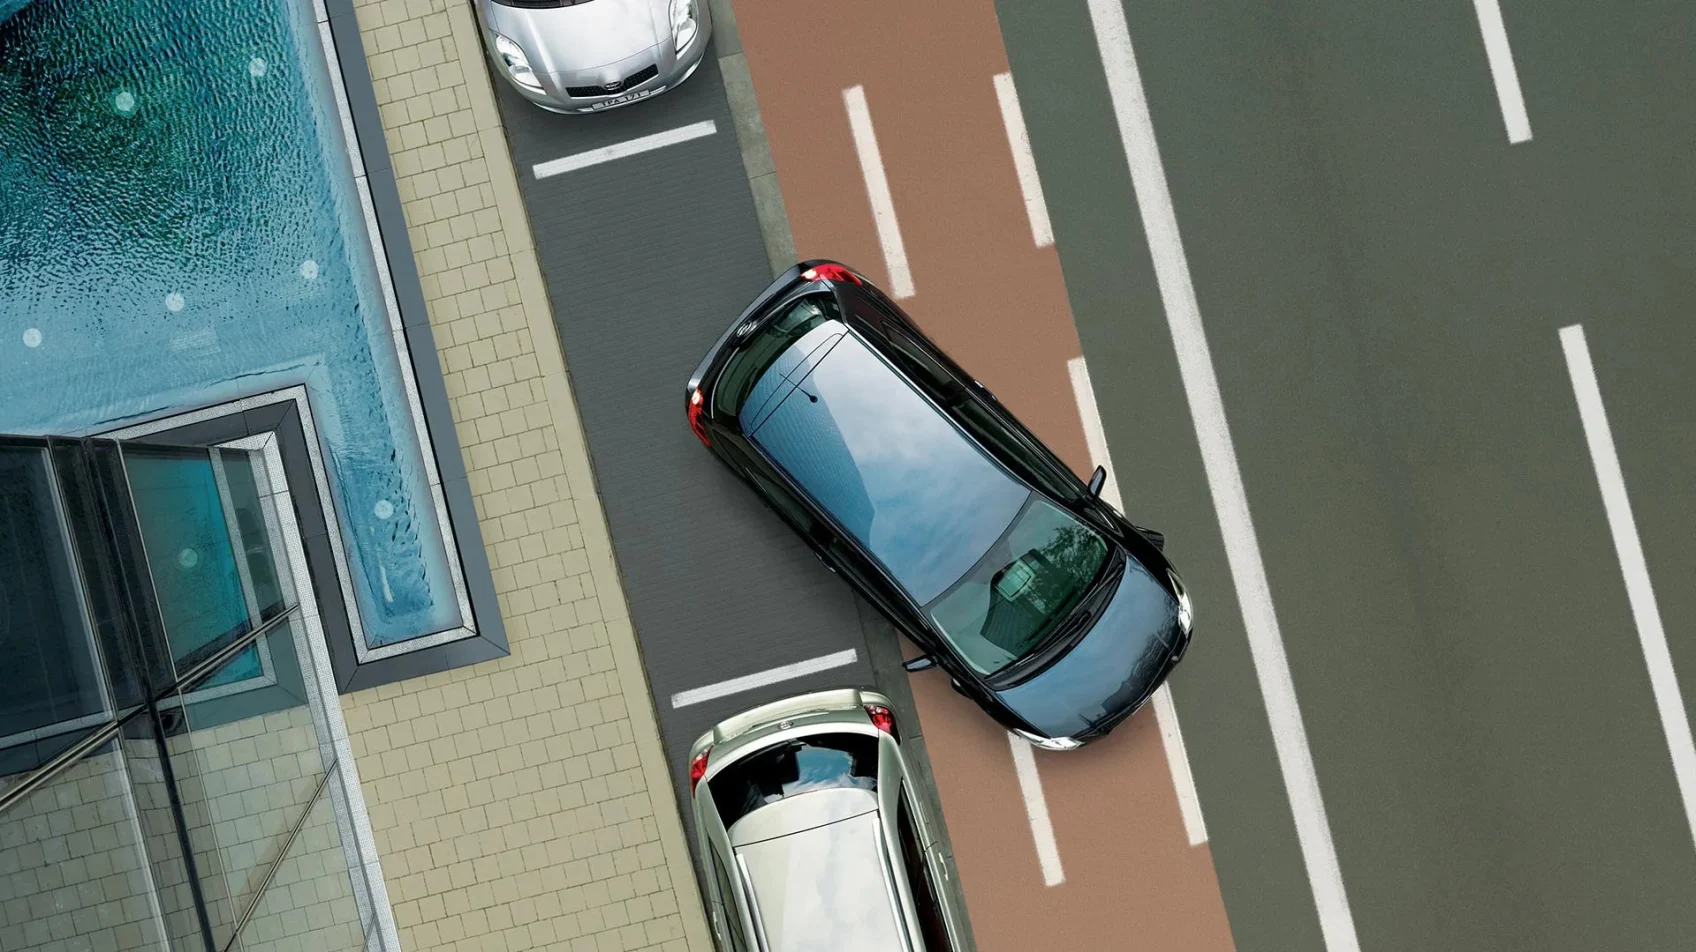
\includegraphics[width=0.80\textwidth]{Resimler/5.png}
\caption{Park Örneği}
\label{fig:5}
\end{figure}

    Sistem, HC-SR04 ultrasonik sensör yardımıyla çevresindeki engellerin mesafesini ölçmekte ve bu verileri işleyerek, uygun park pozisyonunu belirlemektedir. Servo motor, buzzer ve LCD ekranın entegre bir şekilde çalışmasıyla kullanıcıya hem görsel hem de işitsel geri bildirim sağlanmaktadır. Kullanıcıya verilen bu geri bildirimler, park işlemini hem daha hızlı hem de daha güvenli hale getirmektedir.

    Bu çalışma, modern teknolojilerin günlük hayattaki problemleri çözmek için nasıl etkili bir şekilde kullanılabileceğini göstermektedir. Arduino platformunun kullanımıyla oluşturulan bu sistem, düşük maliyetli ve verimli bir çözüm sunarken, aynı zamanda gelecekteki benzer uygulamalar için temel bir prototip olarak işlev görmektedir. Projenin temel amacı, kullanıcıların park etme sürecini kolaylaştırmak, güvenlik risklerini azaltmak ve günlük yaşamda pratik bir yardımcı sistem sunmaktır.

    